\newpage
\section{Resultados}

\subsection*{HPO}
Se encontraron un total de, 45 y 17 genes asociados a los fenotipos tiroiditis (HP:0100646) y Hashimoto (HP:000087) respectivamente.
\subsection*{String}
La red de interacciones obtenida a partir de los 45 genes asociados al fenotipo tiroiditis (HP:0100646), está formada por un total del 122 relaciones, con un grado medio en sus nodos de 5.42 y un coeficiente local de clustering de 0.539 (figura 3.1). Los procesos biológicos (BP, Gene Ontology), funciones moleculares (MF, Gene Ontology) o pathways (P, KEGG) con mejores resultados de anotación (Strenght Log10(observed / expected)) son: (BP, Gene Ontology) Inosine biosynthetic process, (MF, Gene Ontology) Immune receptor activity y (P, KEGG) Non-homologous end-joining , Strenght 2.46, 1.22 y 1.86 respectivamente \cite{StringHP:0100646} \\ \\
La red de interacciones obtenida a partir de los 17 genes asociados al fenotipo hashimoto (HP:000087), está formada por un total del 7 relaciones, con un grado medio en sus nodos de 0.824 y un coeficiente local de clustering de 0.382 (figura 3.2). El pathways (P, KEGG) con mejores resultados de anotación (Strenght Log10(observed / expected) es: (P, KEGG) Inositol phosphate metabolism , Strenght=1.67. \cite{StringHP:0000872} 
\begin{center}
 
    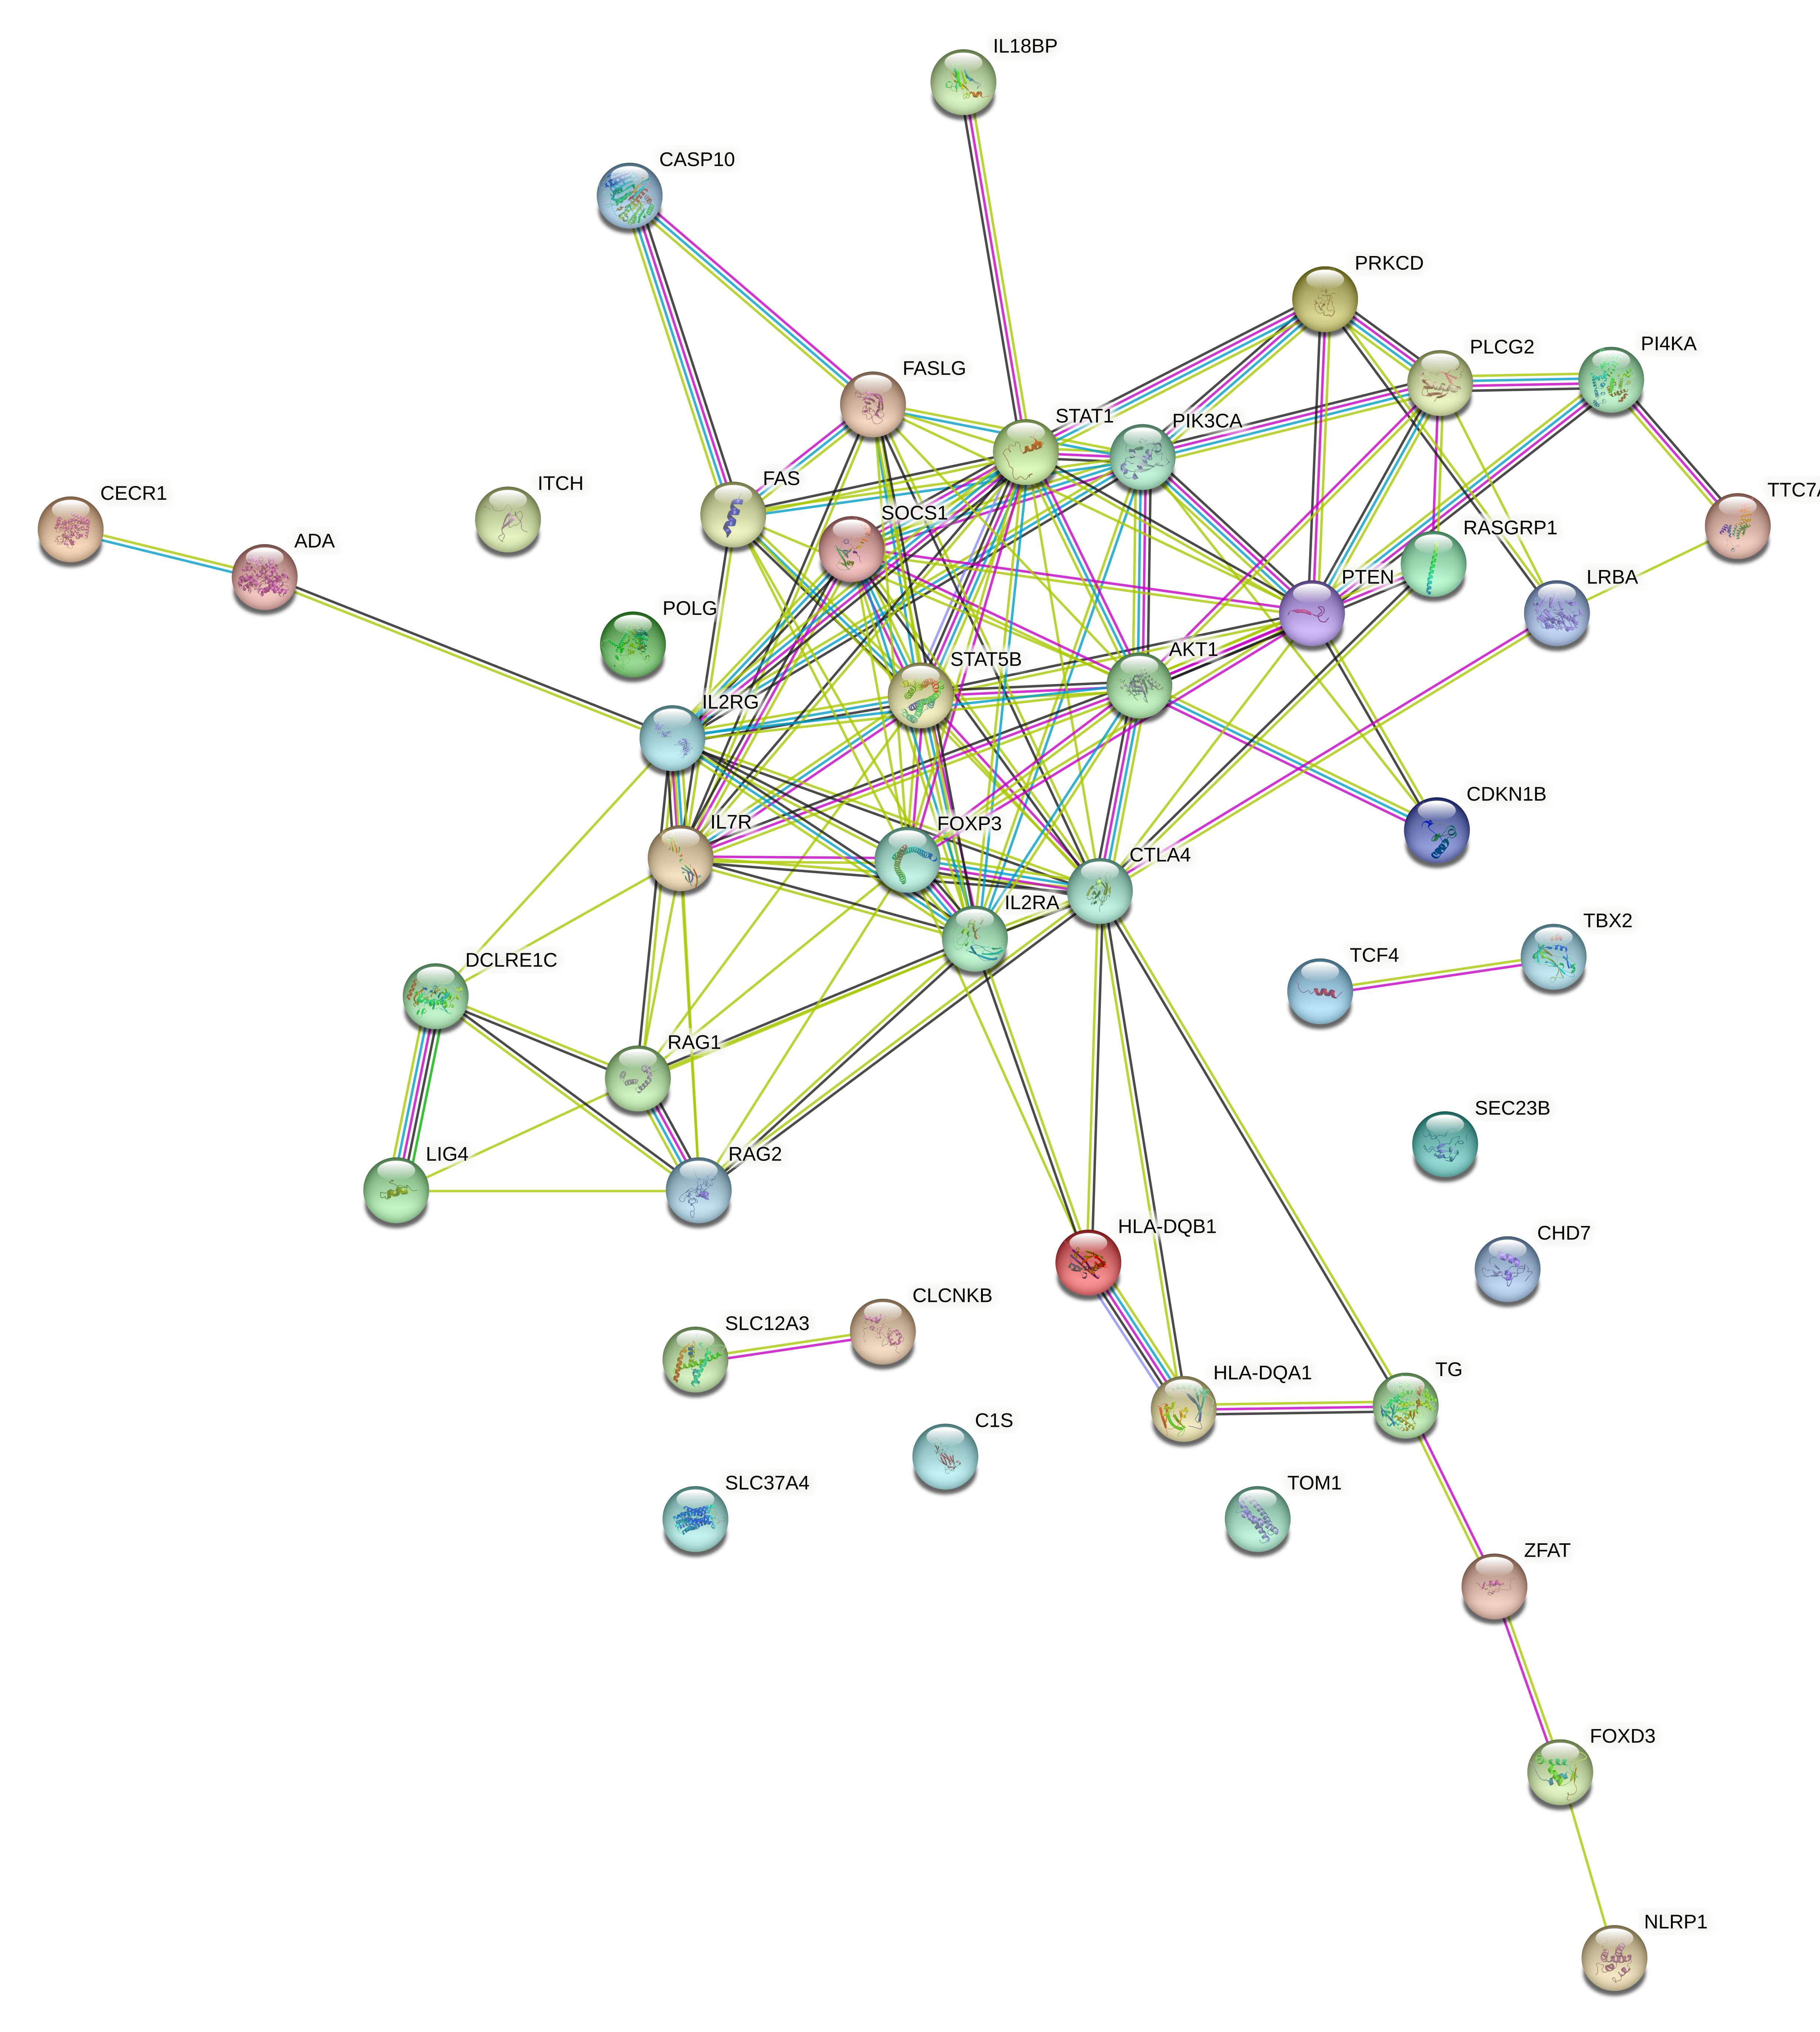
\includegraphics[scale=0.3]{figures/string_thyroiditis.png}
    
    Figure 3.1. Red de Genes HP:0100646
\end{center}


\begin{center}
 
    \includegraphics[scale=0.4]{figures/string_hashimoto.png}
    
    Figure 3.2. Red de Genes HP:000087
\end{center}

\subsection*{Comunidades}
Obtuvimos finalmente los clusters presentes en la red de genes de ambos fenotipos. Los 21 clusters que han sido obtenidos para el fenotipo de tiroiditis se muestran en la figura 3.3.

Los 5 obtenidos para Hashimoto en la figura 3.4.

\begin{center}
 
    \includegraphics[scale=0.5]{figures/comunidades_tiroiditis.png}
    
    Figure 3.3. Dendograma Tiroiditis
\end{center}

\begin{center}
 
    \includegraphics[scale=0.5]{figures/comunidades_hashimoto.png}
    
    Figure 3.4. Dendograma Hashimoto
\end{center}

\subsection*{Análisis Funcional}
Se realizó un análisis funcional (con la terminología KEGG) para identificar en que pathways biológicos intervienen todos los clusters de ambos fenotipos.

\subsection*{Comparación de clusters}
Finalmente, a partir de los pathways comunes obtenidos tras el análisis funcional, hemos determinado los clusters de cada uno de los fenotipos que están implicados en dichos procesos. Estos procesos que hemos obtenido son 'la vía de señalización JAK-STAT' y 'la enfermedad de Alzheimer'. En el primero participan el cluster 2 de Hashimoto y el 11 de Tiroitidis. En el segundo pathway participan el cluster 5 de Hashimoto y el 1 de Tiroiditis.